\chapter{Security of Traffic Control Systems}
\label{chapter:security}

Public traffic infrastructure is arriving in the cyber age with increasing connectivity between the different segments of roadways. For example, freeways are commonly instrumented with loop detectors that allow for real-time monitoring of roadway speeds~\cite{jia2001pems}. Estimates of road traffic conditions are then fed directly into onramp traffic light metering algorithms which regulate traffic flow to improve congestion~\cite{Papageorgiou1991}. Finally, these metering algorithms can be coordinated and controlled by a remote command and monitoring center, leading to a regional network of interconnected sensors and controllers~\cite{Reilly2013b}.

Increased efforts to build systems which understand and utilize the interconnectivity are evidenced by \emph{integrated-corridor-management} (ICM) projects such as \emph{Connected Corridors}~\cite{miller2010san} and mobile applications which use GPS probe data to improve navigation~\cite{work2010traffic}.

This connectivity offers great potential to better analyze, control and manage traffic but also poses a significant security risk. A compromise at any level of the traffic control infrastructure can lead to both direct access of an attacker to alter traffic lights and changeable message signs, and indirect access via spoofing of sensor readings, which may \emph{trick} the control algorithms to respond to false conditions.

A number of traffic-related attacks of infrastructure systems have already been demonstrated in the past few years. A man-in-the-middle attack on GPS coordinate transmissions from mobile navigation applications showed it is possible to trick navigation services into inferring non-existent jams~\cite{jeske2013floating}, while a similar attack used a fleet of mobile phone emulators to mimic the presence of many virtual vehicles on a roadway~\cite{TUFNELL2014}. A popular vehicle-detection sensor was revealed to use a type of wireless protocol vulnerable to data injection attacks, and a demonstration showed that the access point could be tricked into receiving arbitrary readings~\cite{Zetter2014Custom}. Cyber attacks on a centralized command center remain a serious threat given the frequent discovery of networking vulnerabilities, such as the Heartbleed bug~\cite{Codenomicon2014}. Even insider attacks on command centers have precedent as two Los Angeles traffic engineers in 2009 were found guilty of intentionally creating massive delays by adjusting signal times at key intersections~\cite{Grad2009Custom}.

Given the existence of such vulnerabilities and the scale at which they can be exploited, understanding the nature and costs of such attacks becomes paramount to public safety. In this chapter, we present a systematic approach to analyzing the topic of traffic control system vulnerabilities and their potential impact.

To do so, we begin by constructing a taxonomy of different vulnerability locations in traffic control systems, defining three distinct layers: physical, close-proximity, and virtual. Difficulty, impact, and cost values are also associated with each potential attack.  We motivate our classifications by presenting two scenarios that combine a number of attacks to accomplish a high-level goal.

We then focus our analysis on an in-depth exploration of freeway attacks using coordinated, ramp metering. To achieve this, we develop a method based on adjoint computations and finite-horizon optimal control for finding optimal metering rates to create a desired disruption on the freeway. We additionally give an overview of multi-objective optimization and discuss how such an approach is useful for solving high-level attack objectives which contain many conflicting sub-goals, such as permitting a fleeing vehicle to escape pursuants on a particular freeway stretch without overly congesting freeway regions irrelevant to the pursuit.

Central to the plausibility of intricate freeway attacks is the efficiency in which the control and state space of the freeway can be explored. For large systems, brute force exploration would be infeasible, and one could not expect an effective strategy to be computed in a reasonable amount of time. To overcome the large control and state space, this work suggests application of the adjoint method (Chapter~\ref{chapter:adjoint}) and its distributed extension (Chapter~\ref{sec:distributed_optimization_of_coupled_dynamical_systems}) within the multi-objective optimization framework. While the derivations are given explicitly for the centralized form of adjoint control, the methodology extends the distributed case.

The contributions of this chapter are as follows. We present a classification of a broad set of attacks on traffic control systems with their relation to the underlying physical and cyber infrastructure. Mathematical formulations based optimal control and adjoint-based methods are used to show exactly how an attacker can exploit these weaknesses. Explicit algorithms using these tools for coordinated ramp metering attacks are derived and presented. Finally, we provide numerical evidence and novel results of the feasibility of these attacks via simulations modeled after actual freeway networks.

The rest of the chapter is organized as follows. Section~\ref{sec:traffic-system-vulnerabilities} summarizes and classifies the vulnerabilities of traffic control systems. Section~\ref{sec:problemformulation} gives a mathematical approach for carrying out a class of the presented attacks.  Sections~\ref{sub:congestion-on-demand} and~\ref{sub:catchme} give two detailed applications of the mathematical approach to ramp metering attacks. The first application shows how ramp metering can allow an attacker to cause congestion in precise locations and at precise moments in time along a freeway. Simulations are applied to a full-sized model of a 19.4 mile stretch of the I15 South Freeway in San Diego, California. Results are shown for both a custom macroscopic flow simulator as well as an Aimsun~\cite{barcelo2005microscopic} microscopic model. The second application finds a strategy to solve the aforementioned problem of allowing a fleeing vehicles to escape pursuants. Numerical results are presented, as well as a discussion of the benefits of the multi-objective optimization method. We conclude with some future areas of study for traffic system security.


\section{Traffic Control Systems and Vulnerabilities}

In the later part of the chapter we propose attacks to create congestion based on user-defined needs. This section reviews the current architecture of freeway control systems to show that these attacks can be implemented in practice on such systems.

	\subsection{The Freeway Control System}
	\label{sub:freeway-control-system}

	\begin{figure}

	\subfloat[Local freeway control system.] {
	\includegraphics[width=.5\textwidth]{previous-articles/smart-america/diagrams/Catchme-article-diagram-1}
	\label{fig:freewayEntry}
	}
	\hfill
	\subfloat[Global freeway control system.]{
	\includegraphics[width=.5\textwidth]{previous-articles/smart-america/diagrams/Catchme-article-diagram-2}
	\label{fig:globalFreeway}
	}
	\caption[Local and global freeway control system architectures with labeled vulnerability points.]{The physical roadway, sensors, connected vehicles and controllers near a freeway/onramp junction in Figure~\ref{fig:freewayEntry} form a cyber-physical network we refer to as a local freeway control system. The mask icons (white/black masks for indirect/direct vulnerabilities) denote vulnerability points in the local control network.  In Figure~\ref{fig:globalFreeway}, the local controllers are wired together, then connected to a command center via a relay box to form the global control system. This chapter analyzes vulnerability locations associated with each component.}
	\end{figure}
    		Modern freeways encompass control and monitoring mechanisms which enable traffic management to mitigate congestion and improve traffic flow in real-time. While the exact combination of sensors, controllers and transmitters differ from location to location, this chapter chooses one particular instantiation of a freeway control system, which we find to be representative. Figure~\ref{fig:freewayEntry} shows a control system installed near a junction of a freeway and an onramp. We consider three elements of the control system:
    		\begin{itemize}
    			\item Sensors, used to gather information about the freeway state. For example, loop detectors are used to acquire the flow of vehicles along the freeway and onramps/offramps, while the trajectory of vehicles equipped with GPS (or containing GPS-powered smartphone applications) can be used for estimating real-time traffic conditions~\cite{work2010traffic}.
    			\item Actuators, used to influence the evolution and efficiency of the freeway. The most common actuation strategy is \emph{ramp metering}, where traffic lights installed on freeway onramps control the influx of vehicles to the mainline. Other actuators include variable speed limit control~\cite{Muralidharana} and variable message signs. For the purposes of this chapter, the ramp meters are the only actuators we will consider.
    			\item Local controllers, such as \emph{2070} boxes~\cite{AASHTO2012} and the older \emph{170} boxes~\cite{FHWA1978}, which allows interaction between the sensors and ramp meters.
    		\end{itemize}
    		We assume control boxes are wired to the nearby metering light and have a wireless connection to nearby sensors. Vehicles with navigation devices such as TomTom automatically analyze radio-broadcasted traffic reports from traffic control centers to improve their navigating functionality.
    
    		In order to allow coordinated control and sensing across a freeway stretch with many onramps, the local control systems are connected to allow for a more global configuration. Figure~\ref{fig:globalFreeway} depicts our representative global communication architecture. The local control boxes are wired together along the freeway to form the actuation network, with intermediary \emph{relay boxes} allowing for an uplink and downlink to a remote \emph{command center}. The command center contains instrumentation and personnel for monitoring traffic conditions and setting the metering lights accordingly.

\subsection{Vulnerability Classification}
\label{sec:traffic-system-vulnerabilities}

% \subsection{Infrastructure Weaknesses}
    The traffic control infrastructure is built up of several layers and each layer poses individual security risks, starting from tampering with the actual devices, cables or wireless signals, to attacking the software of deployed devices or attacking the command center.
    Attackers can leverage vulnerabilities in the infrastructure to control or disrupt these
    connected systems. Individual attacks can thereby target the physical layer, the
    communication layer, the layer of the control center, or any combination
    thereof.
    
    \emph{Direct physical access:}
    The physical layer is the lowest attackable layer and involves direct access to
    individual wires, opening and accessing the control box, or tampering with
    individual sensors. Physical attacks involve clipping, tampering, removing, or
    replacing of wires or hardware. For instance, copper wire theft near freeways is a common occurrence~\cite{Sutton2014Custom,Rosenberg2014Custom}. Such attacks need low sophistication, are
    easy to carry out, and are hard to protect against as each device must be physically
    protected given that software-based protection is not effective against physical
    attacks. On the other hand, the attack is costly as (i) direct physical access
    is needed, (ii) the attacker is exposed, and (iii) the attack does not scale
    (i.e., each piece of equipment is attacked individually). Examples of such an
    attack in Figure~\ref{fig:freewayEntry} include clipping or removing wires
    between sensors and the \emph{2070} controller, tampering with individual sensors, the
    ramp meter, or the \emph{2070} controller.

\emph{Proximity access (locality):}
Figure~\ref{fig:globalFreeway} depicts multiple control boxes chained together to form a corridor
where actuators have a coordinated plan between the different control
boxes. An attack on the communication layer forges, removes, replaces, or
inserts attacker-controlled measurements into the control system, which may then make further decisions based on forged data. An attacker can either replace or add sensors to
the current sensor network to inject new measurements or attack the software
running on sensors and/or actuators to take over control. Both aspects of the
attack are feasible; the first aspect needs additional hardware and an attacker
that delivers the hardware, the second aspect needs to find a software
vulnerability with a security analysis of the existing devices. These attacks
need higher sophistication and knowledge but no longer need direct hardware
access to the existing sensors and scales to some extent.

\emph{Networked/virtual access:}
Remote connections from the physical freeway infrastructure to the command center defines another layer with potential vulnerabilities. An attack on this layer can be done by forging or controlling messages from/to the command center and
possibly even compromises the command center itself. For this scenario an
attacker needs to find software vulnerabilities in the software running in the
command center. Direct access to these centers is usually not given and this
attack therefore is highly sophisticated (or needs insider access). This attack
is the hardest possible attack as command centers and back links are usually
guarded but allows a great scaling effect as many control boxes can be
controlled directly.

\begin{table}[t]
\centering
\begin{tabular}{p{6cm}llll}
Attack Description & Access & Control & Complexity & Cost \\
\hline
copper theft/clipping wires & physical & low & low & low \\
replacing a single sensor/actuator & physical & low & low & low \\
attacking a single sensor/actuator & locality & low & medium & low \\
replacing a single control box & physical & medium & medium & medium \\
replacing a set of sensors/actuator & physical & medium & medium & medium \\
attacking a set of sensors/actuator & locality & low & medium & low \\
replacing a corridor of control boxes & physical & high & medium & medium \\
attacking a corridor of control boxes & network & high & high & medium \\
attacking the control center & network & high & high & high \\
spoofing GPS data & network & medium & high & medium \\
attacking navigation software & network & medium & medium & medium \\
\end{tabular}
\caption{List of possible infrastructure attacks with access to different layers
that is needed, level of control that the attacker gains, sophistication of the attack, and cost.\label{table:attacks}}
\end{table}

Table~\ref{table:attacks} gives a (partial) list of vulnerabilities in our freeway control system along with classifications for each attack.

\subsubsection{Motivating Examples}

We will consider two fictional but realizable attack scenarios and study their consequences on the compromised network. The first scenario involves indirect control of the freeway, through spoofing the sensors, to achieve a local objective. The second scenario involves direct control of the ramp meters to achieve a global objective along a larger stretch of freeway. 

        The distinction between direct and indirect control is illustrated in Figure~\ref{fig:freewayEntry} via the white mask (indirect) and black mask (direct) icons; direct control can set arbitrary metering rates to a single traffic light or to many lights in a coordinated fashion, while indirect control only modifies sensor readings, with the anticipation that the uncompromised metering system will respond to the spoofed sensors in a predictable manner. Examples of direct attacks include a compromise of the \emph{2070} boxes which are directly wired to the meters and a compromise of the command center, which issues upstream metering plans to the \emph{2070} controllers. Examples of indirect attacks include sending fake loop-detector readings to access points and broadcasting false traffic reports to GPS devices which may respond with poor routing advice.

\paragraph{Direct Attack: catch-me-if-you-can}
            \label{sss:catchmescen}
            The objective of the attacker is to escape from pursuants along a large section of freeway. A compromise of all the ramp meters is assumed, as it permits the attacker to selectively congest certain sections of the roadway (see Section~\ref{sec:problemformulation}).  One approach is to hack the command center itself, with the downside being the expensiveness and complexity of such an attack (see Table~\ref{table:attacks}). Another solution is to begin by hacking one of the \emph{2070} boxes, and since all the \emph{2070} boxes are networked along the freeway (see Figure~\ref{fig:globalFreeway}), a single hacked box can serve as a means of compromising the other nearby boxes, leading to a cascading attack. The attacker can then acquire full control of all the \emph{2070} boxes, and in turn, the ramp metering lights.
            \\
            The current traffic control architecture presented above supports the class of attacks described in the next section. Specifically, a mathematical approach to coordinated ramp metering attacks is developed to permit an attacker to effectively exploit vulnerabilities in the metering control system.

\paragraph{Indirect Attack: VIP-lane}

\begin{figure}[t]
    \centering
    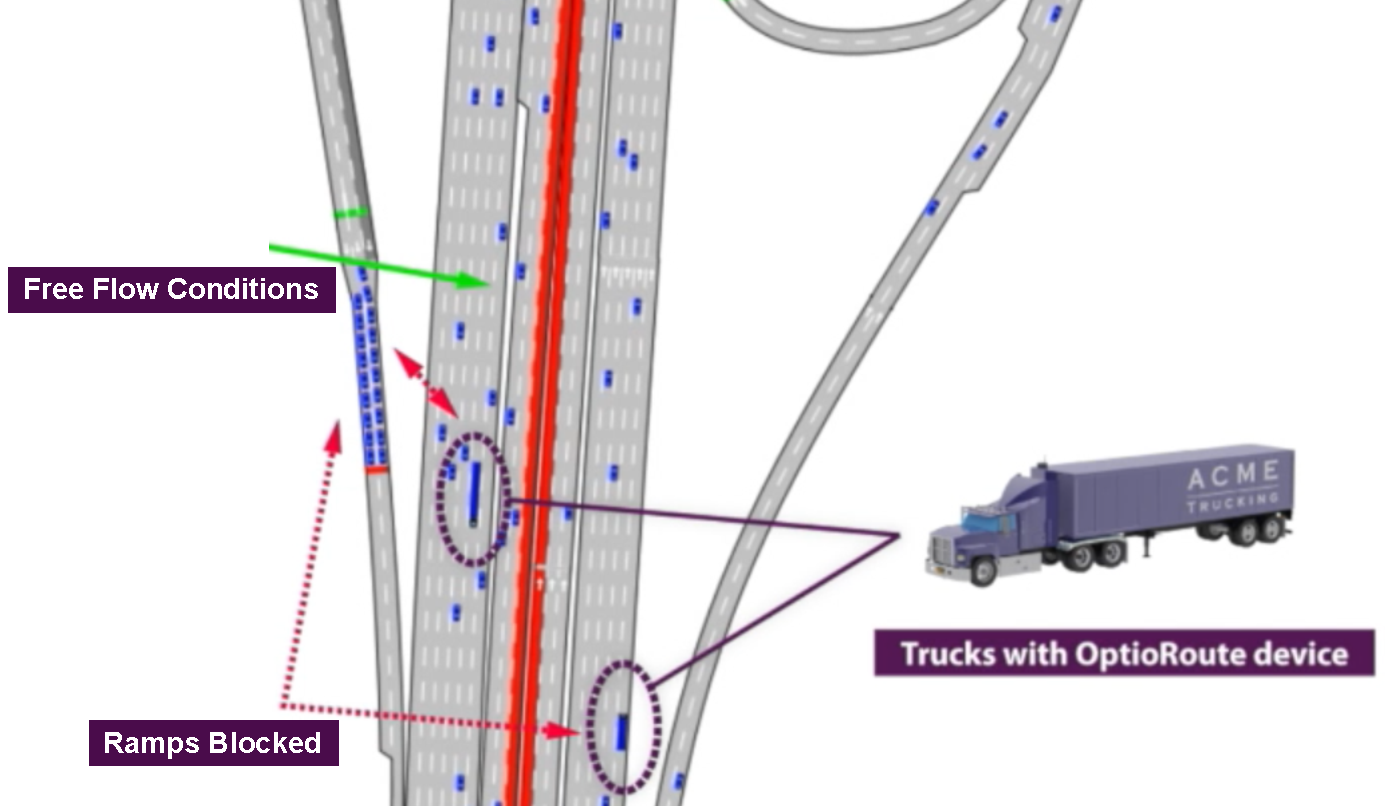
\includegraphics[width=0.7\textwidth]{diagrams/trucks}
    \caption[Diagram of the VIP-Lane attack on the Aimsun micro-simulation.]{Diagram of the VIP-Lane attack on the Aimsun micro-simulation. Trucks (dramatized in~\cite{smartroadswebsite} as belonging to a hypothetical delivery company, OptiRoute) passing by transmit fake traffic count data in an attempt to spoof the readings received by the traffic count sensors. The count sensors are deceived into inferring high-density conditions, causing large amounts of metering on the on ramps while creating free-flow conditions on the mainline.}
    \label{fig:smart-roads-diagram}
\end{figure}


            The objective of the attacker is to clear a predetermined section of a regularly congested freeway. The attacker drops low-cost wireless transmitters near the \emph{2070} controllers along the freeway section. As the actual loop-detector sensors communicate with the control box wirelessly, the attacker will be able to override the loop-detector signals and send false data that indicates a fully congested freeway. This will indirectly affect the ramp meters, which will respond by limiting on ramp flow and thus eliminating significant freeway mainline flow. The attacker will then transmit false GPS location data via a set of hacked cellphones to trick navigation software into believing the freeway is congested. Approaching vehicles using navigation software will then be rerouted around the fake congestion which leads to a further reduction in incoming flow. The net effect of the attack is a congestion-free commute for the attacker: a private VIP lane created purely by indirect, sensor-based attacks.

A depiction of the VIP-lane attack is shown in Figure~\ref{fig:smart-roads-diagram}. The attack was also implemented numerically as a part of the SmartRoads project, which is discussed in the next section.

\subsection{SmartRoads and SmartAmerica}

\begin{figure}[t]
    \centering
    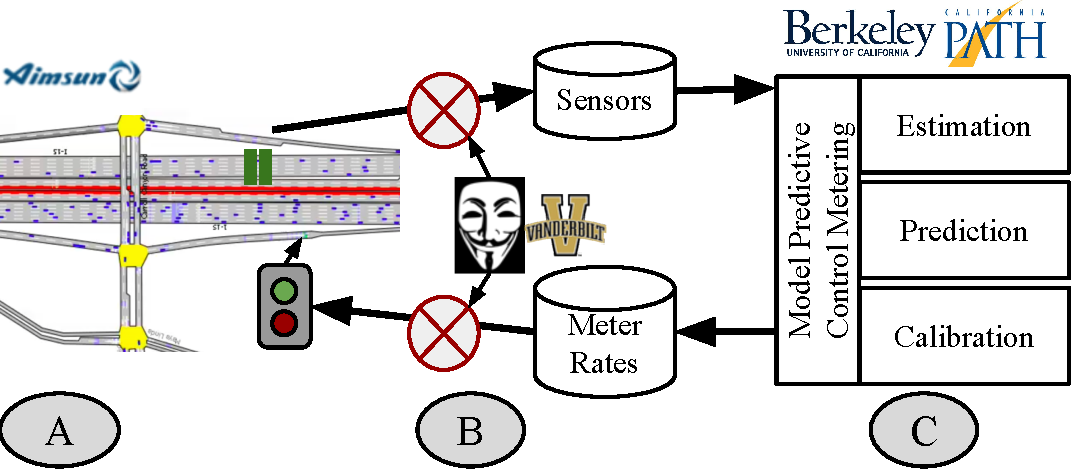
\includegraphics[width=0.95\textwidth]{diagrams/smart-roads}
    \caption[System diagram for SmartRoads project depicting Aimsun microsimulator, Connected Corridors system, and C2WindTunnel software.]{System diagram for SmartRoads project. The Aimsun micro-simulator (Label A) interfaces with the Connected Corridors Control System (Label B) through databases. The C2WindTunnel (Label C) system models networking and serves as the attack point. Sensors information intercepts are indirect attacks, while metering command intercepts are direct attacks.}
    \label{fig:smart-roads-truck}
\end{figure}

As part of the White House SmartAmerica 2014 Conference on cyber-physical systems, A UC Berkeley PATH institute and Vanderbilt University collaboration presented a functional microscopic simulation framework for conducting and analyzing cyber attacks on freeway control infrastructure. The project, nicknamed SmartRoads, consists of three main components:

\begin{itemize}
    \item UC Berkeley \emph{Connected Corridors}: A simulation and decision support system for traffic systems which implements estimation and ramp metering control.
    \item TSS Aimsun~\cite{barcelo2005microscopic}: a microscopic traffic simulator with API's for broadcasting loop-detector information and modifying metering rates dynamically.
    \item Vanderbilt C2WindTunnel~\cite{chabukswar2010simulation}: A computer network communication simulator and visualization tool.
\end{itemize}

The ultimate mission of the collaboration is to allow for a comprehensive modeling of traffic control system vulnerabilities to enable real-time security compromise detection and prevention. SmartRoads aims to accomplish this by modeling the flow of information and communication between the Connected Corridors system and the Aimsun simulator.

As a initial task, a simulation of both indirect and direct attacks was conducted on a calibrated microscopic model of the I15 Freeway. As the communication between Aimsun and Connected Corridors is conducted through database intermediaries, the C2WindTunnel software was installed on the communication link between Aimsun and the databases. Before sensor information reached the database from Aimsun and before metering commands reached Aimsun from the database, C2WindTunnel simulated a communication interception and modified the contents of the packets. A sensor intercept is viewed as a simulated indirect attack, while a metering rate intercept is viewed as a simulated direct attack. The system architecture of SmartRoads is summarized in Figure~\ref{fig:smart-roads-truck}.

The VIP-Lane attack was fully simulated on the SmartRoads system, where a video playback of the simulation clearly indicates that a spoofing attack on the loop detectors results in an under-utilized freeway mainline, while the metering algorithms are ``tricked'' into over-metering.  See our link~\cite{smartroadswebsite} for a Youtube video depiction.

A direct attack was also simulated in the SmartRoads framework, demonstrating the interception of metering commands to a series of traffic lights along I15 South. The attack, referred to as a \emph{box attack}, attempts to create a precise pocket of congestion over a predetermined section of road and period of time. The details of box attacks, as well as a visual summary of the direct attack within SmartRoads, are given in Section~\ref{sub:congestion-on-demand}.


\section{Coordinated Ramp Metering Attacks}
\label{sec:problemformulation}

An attacker can negatively influence the performance of the freeway network or achieve some criminal goal by setting the metering lights to a particular configuration. The impact of such an attack can be maximized by leveraging a discrete dynamical freeway model to compute metering rates which achieve the desired goal using finite-horizon optimal control and multi-objective optimization techniques.

\subsection{Optimal Control Model}
\label{sub:fhoc-adjoint}

\subsubsection{Optimal Control Formulation}

Using the discrete model in Section~\ref{sec:continous-and-discrete-traffic-model-for-ramp-metering} mathematically expressed as follows:

\begin{align}
    \delta\left[i,k\right] & = \min\left(v \rho\left[i,k\right], f^{\max} \right) \\
    \sigma\left[i,k\right] & = \min\left(w\left(\rho^{\max} - \rho\left[i,k\right]\right), f^{\max}\right) \\
    d\left[i,k\right] & = u\left[i,k\right]\min \left(l\left[i,k\right] / \triangle t, r^{\max}\right) \\
    f^{\text{in}}\left[i,k\right] & = \min\left(\sigma\left[i,k\right], d\left[i-1,k\right] + \beta\left[i,k\right] \delta\left[i,k\right]\right) \\
    f^{\text{out}}\left[i,k\right] & = 
    \begin{cases}
    \delta\left[i,k\right] & \quad \mbox{if } \frac{p f^{\text{in}}\left[i+1,k\right] }{\beta\left[i,k\right] \left(1 + p\right)} \ge \delta\left[i,k\right] \\
    \frac{f^{\text{in}}\left[i+1,k\right] - d\left[i+1,k\right]}{\beta\left[i,k\right]} & \quad \mbox{if } \frac{f^{\text{in}}[i+1,k]}{1 + p} \ge d\left[i+1,k\right] \\
    \frac{p f^{\text{in}}\left[i+1,k\right]}{\left(1 + p\right) \beta\left[i,k\right]} & \quad \mbox{otherwise}
    \end{cases} \\
    r\left[i,k\right] & = f^{\text{in}}\left[i,k\right] - \beta\left[i,k\right] f^{\text{out}}\left[i,k\right] \\
    \rho\left[i,k+1\right] & = \rho\left[i,k\right] + \frac{\triangle t}{\triangle x} \left(f^{\text{in}}\left[i,k\right] - f^{\text{out}}\left[i,k\right]\right)\\
    l\left[i,k+1\right] & = l\left[i,k\right] + \triangle t \left(D\left[i,k\right] - r\left[i,k\right]\right),
\end{align}

we seek a method to compute a coordinated ramp metering policy $u\left[i,k\right]$ over all space $i\in\left[1,N\right]$ and time $k\in\left[1,T\right]$, which minimizes (or reduces) some specified objective. We cast the problem as a finite-horizon optimal control problem, as done in Section~\ref{par:Optimization-Problem}.

We succinctly express the discrete, controllable dynamical system given in Section~\ref{sec:continous-and-discrete-traffic-model-for-ramp-metering} by:
	\begin{equation}
	\label{eq:concat-sys}
		H\left(\vectorize{u}, \vectorize{\rho}\right)=0.
	\end{equation}

Given some objective function $J\left(\vectorize{u}, \vectorize{\rho}\right)$, our goal is now to find the optimal $\vectorize{u}^*$ which solves the following constrained \emph{finite-horizon optimal control} problem:
	\begin{align}
		\label{eqn:fhoc}
		\min_{u} \;& J\left(\vectorize{u}, \vectorize{\rho}\right) \\
		\text{subject to:} \;& Equation~\eqref{eq:concat-sys} \label{eqn:repeat-concat-system}.
	\end{align}

We utilize the discrete adjoint method discussed in Section~\ref{sec:discrete-adjoint-method} to efficiently compute gradients within a first-order descent method.

\subsection{Multiple Objectives: Interactive Multi-objective Optimization}
	\label{sub:moo}
		A high-level attack goal often requires satisfaction of many \emph{sub-goals} at once, and often-times the sub-goals can be competing or conflicting. For example, in the \emph{catch-me-if-you-can} scenario, the attacker wants to escape from his chasers. Hence the attacker wants to travel the freeway as quickly as possible, but also wants to slow down the chasers behind. As a consequence, we have two simpler but competing objectives.

		Such a situation with multiple, competing objectives can be described as a \emph{multi-objective optimization problem}.

		\subsubsection{Multi-objective Optimization and Pareto Front}
			\begin{definition}[Multi-objective optimization problem]
			Given $N \in \mathbb{N}$, let $ ( f_i\left(\vectorize{u}, \vectorize{\rho}\right))$ be a set of $N$ objective functions describing the goal of a freeway attack. The \emph{multi-objective optimization problem} we consider is the following simultaneous minimization problem:
				\begin{equation}\label{eq:multiobj_def}
						\min_{x\in X} \; \left(f_1(x), f_2(x),\ldots, f_N(x) \right)
				\end{equation}
			\end{definition}
			As we are now minimizing a vector and not a scalar, we need to define how a solution of equation~\eqref{eq:multiobj_def} can be ``better'' than another.

			\begin{definition}[Pareto front]\label{def:paretofront}
			An solution $x \in X$ is said to \emph{Pareto dominate} another solution $x'$ if:
				\begin{itemize}
						\item $\forall i \leq N \quad f_i(x) \leq f_i(x')$
						\item $\exists j \leq N \quad f_j(x) < f_j(x')$
				\end{itemize}
			A solution $x \in X$ is called \emph{Pareto optimal} if there is no other solution $x'$ that dominates it. The set of all Pareto-optimal solutions is called the \emph{Pareto front}, $P \subseteq X$.
			\end{definition}

			Hence, we consider Pareto-optimal solutions to be the solutions of Equation~\eqref{eq:multiobj_def}.

			\subsubsection{Decision Maker}
			There are many ways to find a Pareto-optimal solution. For example if we have three objective functions, we can minimize $f_1$ first, minimize $f_2$ on the subset $\argmin_{x \in X} f_1(x)$ and finally minimize $f_3$ on the remaining subset to obtain a Pareto-optimal solution. But we could also do the same in any order, with potentially very different results. Thus, the Pareto front can sometimes be very large and hard to explore. As a consequence, we need to be able to identify the most desirable solutions within the potentially large Pareto front.

			
			A \emph{Decision Maker} (DM) represents the human whose expertise is used to discern a preference between two control values. As we only wish to judge controls which are Pareto optimal, The DM only observes and discerns values on the Pareto front to limit the search space and improve the efficiency of the method. As a consequence, the DM has a hidden objective function: $u\left(\vectorize{u}, \vectorize{\rho}\right)$, the \emph{utility function}, which can only be indirectly observed through probing the DM. With $u$, we can reformulate the multi-objective optimization problem as:
			\begin{equation}\label{eq:multiobj_dm}
					\min_{x\in P} \;u(x)
			\end{equation}

			The DM is essential to multi-objective optimization problems with large Pareto fronts.  There are several ways to interact with him:
			\begin{itemize}
				\item He can evaluate his utility function $u$ on any given Pareto-optimal solution.
				\item He can give more general preferences on the Pareto front, for example a preference for one of the objective functions, or for a given subset of the Pareto front.
			\end{itemize}

			
		\subsubsection{Finite-horizon Optimal Control and Multi-objective Optimization}
			\paragraph{Scalarization}
In order to find Pareto-optimal solutions, we will reduce the problem to the common scalar minimization problem, which can be solved with the optimal control tools of Section~\ref{sub:fhoc-adjoint}. This process is called \emph{scalarization}. As our particular scalarization, we use a linear combination of the individual objective functions:

\begin{equation}
\label{eqn:linear-combo}
f(x) = \sum_{i \leq N} a_i f_i(x).
\end{equation}

The DM can favor a specific objective $f_i$ over other objectives by increasing the $a_i$ coefficient.

It is easy to show that any solution of Equation~\eqref{eqn:linear-combo} will also belong to the Pareto front. As a consequence, we can explore at least a subset of the Pareto front (with the hope that this subset is representative) by minimizing a linear combination of the objective functions.


For example, the next proposition shows that a linear combination of the objectives is a type of scalarization.
\begin{proposition}
\label{prop:scalarization}
	If a solution $x \in X$ satisfies: 
	\begin{equation}\label{eq:linear_combination}
		\exists \; (a_i)_{i\leq N} \in \mathbb{R}_{+}^*\qquad x \in \argmin_{y \in X} \sum_{i \leq N} a_i f_i(y)
	\end{equation}
	Then x is a Pareto optimal solution
\end{proposition}
\begin{proof}
	If $x$ is not a Pareto optimal solution, a solution $y \in X$  Pareto - dominate $x$, by Definition~\ref{def:paretofront}. As a consequence, we have:
	\begin{itemize}
			\item $\forall i \leq N \quad f_i(y) \leq f_i(x)$
			\item $\exists j \leq N \quad f_j(y) < f_j(x)$
	\end{itemize}
	And immediately:
	\begin{equation*}
		\sum_{i \leq N} a_i f_i(y) \quad < \quad \sum_{i \leq N} a_i f_i(x)
	\end{equation*}
	So $x \not \in \argmin_{y \in X} \sum_{i \leq N} a_i f_i(y)$, hence the proof by contraposition.
\end{proof}

			\paragraph{A Posteriori Method}
				Equation~\eqref{eqn:linear-combo} allows one to sample the Pareto front by exploring the space of the coefficients which can provide to the DM a representative subset of Pareto-optimal solutions. The DM can then choose {\it a~posteriori} his preferred solutions. And as such this method is called an \emph{a~posteriori method}.

				This method can be computationally costly as many different optimal control problems need to be solved, but provides a good overview of the Pareto front. In particular, it gives an estimation of the lower and upper bounds of each objective function. Thus one can scale each objective function to take values only between 0 and 1, allowing the different objectives to be easily compared.
			\paragraph{Interactive Method}
				\begin{figure}[ht]
					\centering
					  \includegraphics[width=.7\textwidth]{previous-articles/smart-america/diagrams/interactive}
					\caption[The interactive method for multi-objective optimization embeds the Decision Maker (DM) in the optimization loop, allowing the DM to direct the search of the Pareto front.]{The interactive method for multi-objective optimization embeds the Decision Maker (DM) in the optimization loop, allowing the DM to direct the search of the Pareto front. The optimal controller adapts the advice of the DM to \emph{scalarize} the multiple objectives and solve a new optimization problem. The results of the optimization are then fed back to the DM, and the cycle repeats until satisfaction.}
					\label{fig:interactive}
				\end{figure}
				Unlike with the a~posteriori method, \emph{Interactive methods} are based upon a repeated interaction with the Decision Maker.
				\begin{enumerate}
					\item The DM gives an indication of how to compute the next Pareto-optimal solution --- for example, he may give an idea for the next set of coefficients $(a_i)$ to use and his evaluation of the previous simulation.
					\item The interactive scalarization process uses this indication to create a scalar objective --- for example using Equation~\eqref{eqn:linear-combo}, we obtain a scalar objective with the set of coefficients given by the DM.
					\item The finite-horizon optimal control method is used to solve the corresponding optimization problem, and gives the result to the DM.
				\end{enumerate}
				This process is repeated until the DM is satisfied with the results. Figure~\ref{fig:interactive} shows the general process of interactive methods.

				The important part of the interactive method is the kind of indications that can be given by the DM, and how the indications and the simulation history will be used in the scalarization process. Section~\ref{sub:catchme} gives an example of an interactive method.

\subsection{Congestion-on-demand Attack}
\label{sub:congestion-on-demand}

We will now apply the tools of \emph{adjoint-based finite-horizon optimal control} and \emph{multi-objective optimization} from Section~\ref{sec:problemformulation} to two families of attacks. The first attack highlights the precision of coordinated ramp metering attacks, while the second showcases the benefits of multi-objective optimization.

Following reproducible research practices~\cite{donoho2009reproducible,stodden2009enabling}, the software and data used to produce the numerical results and diagrams in this section is made available~\cite{smartroadswebsite} to permit the reader to reproduce the presented results.

\subsubsection{Simulation Network}

The attacks for the first example, \emph{box objective} (to be described), use a macroscopic freeway model of a 19.4 mile stretch of the I15 South Freeway in San Diego California. The model was split into 125 links with 9 onramps and was calibrated~\cite{dervisoglu2014macroscopic,Muralidharan2009c} using loop-detector measurements available through the PeMS loop-detector system~\cite{jia2001pems}. Figure~\ref{fig:i15} is a \emph{Space-time diagram} of the I15 freeway. There is no ramp metering control applied to the simulation in Figure~\ref{fig:i15}, i.e. the ramp meters are always set to green.

\begin{figure}
\centering
\subfloat[Simulation with no metering.]{
  \includegraphics[width=.55\linewidth]{previous-articles/smart-america/diagrams/I15preshack}
  \label{fig:i15}
}\\
\subfloat[Trade-off: $\alpha = 0.3$] {%
  \includegraphics[width=.32\linewidth]{previous-articles/smart-america/diagrams/box3hack}%
  \label{fig:box3}%
}\hfill
\subfloat[Trade-off: $\alpha = 0.5$] {%
  \includegraphics[width=.32\linewidth]{previous-articles/smart-america/diagrams/box5}%
  \label{fig:box5}%
}\hfill
\subfloat[Trade-off: $\alpha = 0.9$] {%
  \includegraphics[width=.32\linewidth]{previous-articles/smart-america/diagrams/box9}%
  \label{fig:box9}%
}%
\caption[I15 South box objective attack with multiple trade-off parameter values.]{Figure~\ref{fig:i15} depicts a space-time diagram of vehicle densities on 19.4 mile stretch of I15 Freeway with no ramp metering. The box objective, and example of \emph{congestion-on-demand}, is applied in Figures~\ref{fig:box3}-\ref{fig:box9}. The user specifies a ``desired'' traffic jam between postmile 4.5 and 14, for a duration of 20 minutes between 8:20 and 8:40. For this, the $\alpha$ parameter (introduced in Equation~\eqref{eqn:alpha}) enables the proper design of tradeoffs in the objective.}
\end{figure}

\subsubsection{Constructing the objective function}
In order to achieve the \emph{congestion-on-demand} objective, we will use the finite-horizon optimal control technique introduced in Section~\ref{sub:fhoc-adjoint}. Therefore, we need to create a class of objective functions able to represent any jam pattern on the freeway. The method we have chosen is to maximize the traffic density where we want to put the congestion, while minimizing it everywhere else.

For every cell density value at position $i$ and time $k$, we assign a coefficient $a_i^k \in \mathbb{R}$. We can then define the corresponding objective function:
\begin{equation}
\label{eqn:jamondemand}
J \left( \vectorize{u}, \vectorize{\rho} \right) = \sum_{i = 1}^{N} \sum_{k = 1}^{T} a_i^k \, \rho\left[i,k\right]
\end{equation}
When $J$ is minimized, a positive coefficient $a_i^k$ will encourage the minimization of the traffic density at position $i$ and time $k$, whereas a negative coefficient will encourage congestion. The absolute value of the coefficient represents the importance given to the fulfillment of the objective at the particular time and location of the simulation.

\subsubsection{Congestion On Demand Examples}

\paragraph{Box Objective}
The \emph{box objective} creates a box of congestion in the space-time diagram, i.e. congestion will be created on a specific segment of the freeway during a user-specified time interval.


As we have two competing goals (maximize congestion in the box, minimize congestion elsewhere), we apply the multi-objective optimization procedure in Section~\ref{sub:moo}. Indeed, we have the following two objective functions:
\begin{align}
	f_1 \left( \vectorize{u}, \vectorize{\rho} \right) & = - \sum_{(i,k) \in \text{Box}} \rho\left[i,k\right] \\ 
	\text{and} \; f_2 \left( \vectorize{u}, \vectorize{\rho} \right) & =  \sum_{(i,k) \not \in \text{Box}} \rho\left[i,k\right]
\end{align}
To solve this multi-objective problem, we balance our two objectives using a linear combination. As we limit ourselves to one degree of freedom, we introduce a single parameter $\alpha \in \left[0,1\right]$ and minimize the following objective function:
\begin{equation}
\label{eqn:alpha}
J_{\alpha} \left( \vectorize{u}, \vectorize{\rho} \right) = \alpha \, f_1 \left( \vectorize{u}, \vectorize{\rho} \right) \: + \: \left(1 - \alpha \right) \, f_2 \left( \vectorize{u}, \vectorize{\rho} \right),
\end{equation}
where $\alpha$ is a trade-off parameter: $\alpha = 1$ is complete priority on the congestion inside the box, while $\alpha = 0$ is complete priority on limiting density outside the box.


The results of the box objective are presented in Figures~\ref{fig:box3}-\ref{fig:box9}. We give space-time diagrams for three different values of the parameter $\alpha$. The box of the objective is shown as a black frame with an actual size of 10 miles and 20 minutes. As the trade-off moves from $\alpha=0.3$ to $0.9$, there is a clear increase in the congestion within the box, at the expense of allowing the congestion to spill outside the desired bounds. In fact, Figure~\ref{fig:box9} ($\alpha=0.9)$ activates the bottleneck near the top-left of the box earlier than Figure~\ref{fig:box3} ($\alpha=0.3$) to congest the middle portion of the box, which leads to a propagation of a congestion wave outside the bounds of the bottom-right of the box.

\begin{figure}
	\centering
	\includegraphics[width=0.95\textwidth]{previous-articles/smart-america/diagrams/boxi15aimsun}
	\caption[Box objective attack implemented on a microscopic model of I15 Freeway produced with Aimsun software.]{Box objective attack implemented on a microscopic model of I15 Freeway produced with Aimsun software.  The metering lights were set using the \emph{congestion-on-demand} strategy. Snapshots of traffic at the north and south extents of the box show that the strategy maintains congestion within the box and free-flow conditions outside the box. A link to a video of the microsimulation is provided~\cite{smartroadswebsite}. Best viewed in color.}
	\label{fig:boxi15aimsun}
\end{figure}

As a part of the SmartRoads project, we also implemented the box objective on an Aimsun microsimulation model~\cite{barcelo2005microscopic} of the I15 freeway network. This model originates from the I15 integrated corridor management project ran in San Diego in 2010, ref~\cite{miller2010san}. The geographical location of the I15 network is given in Figure~\ref{fig:boxi15aimsun} and shows San Marcos as the southbound start and Mira Mesa as the end, with the desired box of congestion placed approximately 5 miles before Mira Mesa. A snapshot of the northern and southern extents of the box at the time of 8:30 are shown below the map. The south-bound lanes in the snapshot indicate that congestion was more or less confined to the desired box. A summary video~\cite{smartroadswebsite} of the I15 microsimulation shows the formation and dissipation of congestion within the predetermined freeway section.

\paragraph{Attack to Create Traffic Patterns in the Form of Morse Code}

\begin{figure}[h]%
\centering%
\subfloat[Space-time diagram.]{%
  \includegraphics[width=.55\textwidth]{previous-articles/smart-america/diagrams/calmorsewithoutcal}%
  \label{fig:calmorsespacetime}%
}\hfill%
\subfloat[Density profiles over space for three moments in time spaced 17 minutes apart. Best viewed in color.]{%
	\includegraphics[width=.42\textwidth]{previous-articles/smart-america/diagrams/cal-morse-freeway}%
	\label{fig:calmorseslices}%
    }
\caption[Attack to create traffic patterns in the form of Morse code. A coordinated ramp metering attack using the proposed algorithm is able to spell out ``C-A-L'' in Morse code over successive time-slices of the space-time diagram.]{Attack to create traffic patterns in the form of Morse code. A coordinated ramp metering attack using the proposed algorithm is able to spell out ``C-A-L'' in Morse code over successive time-slices of the space-time diagram: C$=- \cdot - \cdot$, A$= \cdot -$, L$= \cdot - \cdot \cdot$. The entire space-time diagram of the attack is shown in Figure~\ref{fig:calmorsespacetime}, while three snapshots of the freeway are shown in Figure~\ref{fig:calmorseslices}, each slice spelling out one of the letters in ``C-A-L'' in blocks of congestion.}
\label{fig:cal_morse}
\end{figure}

\begin{itemize}
	\item \textbf{Network}
	Since the I15 network does not have enough controllable onramps for the following attacks to be precise, we now consider a 60 mile freeway network with onramps and offramps spaced every 3.75  miles and a fixed demand on the onramps.
	\item \textbf{Attack}
	Figure~\ref{fig:cal_morse} represents the space-time diagram of a \emph{Morse code attack}. The objective is to create the Morse code representation of the three letters ``C-A-L''\footnote{Short for University of California.}, spelled with congestion blocks on the freeway. The corresponding objective function is the superposition of several box objectives on three thin time stripes of the space-time diagram. Everywhere else, the coefficients are put to zero. The result demonstrates that even with a reasonable number of ramps, one can achieve complex attack patterns. In particular, the optimal control approach was able to identify that creating a single backwards-moving jam was the most effective way to produce the second dash for ``C'', the first dash for ``A'' and the first dot for ``L''.
\end{itemize}

\paragraph{Arbitrary Patterns}

\begin{figure}[htbp]
	\centering
	\includegraphics[width=0.95\textwidth]{previous-articles/smart-america/diagrams/flow-arbitrary}
	\caption[Flow-chart for converting an arbitrary image to a \emph{congestion-on-demand} goal.]{Flow-chart for converting an arbitrary image to a \emph{congestion-on-demand} goal. ``Converting'' an objective of the form in Equation~\ref{eqn:jamondemand} allows an attacker to compute metering rates that produce space-time diagrams resembling the original image.}
	\label{fig:flow-arbitrary}
\end{figure}

Provided the right controllability conditions are satisfied, any congestion pattern may be created if the network has enough control ramps. To work towards this, we can choose the negative and positive coefficients of the \emph{congestion-on-demand} method carefully to match a desired pattern. The following process, as depicted in Figure~\ref{fig:flow-arbitrary}, gives a methodological approach to constructing arbitrary \emph{congestion-on-demand} patterns.

One selects some image file they wish to reproduce in congestion patterns on a space-time diagram. The image is thresholded by color intensity to produce a bitmap of regions of desired congestion (X's) and free-flow (O's). Then a \emph{congestion-on-demand} objective (Equation~\eqref{eqn:jamondemand}) is constructed from the bitmap and scalarized using the $\alpha$ balance parameter to produce the $a_i^k$ coefficients. A metering policy minimizing the objective is then computed using the optimal control method in Section~\ref{sub:fhoc-adjoint}. Given sufficient control of the network and optimization time, the resulting space-time diagram from the metering policy will resemble the input image file.

\begin{figure}[ht]
\centering
  \includegraphics[width=1\textwidth]{previous-articles/smart-america/diagrams/cal_logohack}
\caption{Space-time diagram obtained following a \emph{congestion-on-demand} attack with a Cal logo as the objective function. The attack was simulated on a 90 miles and 33-onramp freeway, for a 2 hours simulation time and using coordinated ramp metering.}
\label{fig:cal_logo}
\end{figure}

We give an example of the arbitrary \emph{congestion-on-demand} attack in Figure~\ref{fig:cal_logo}, which produces a space-time diagram resembling the~\raisebox{-1ex}{\includegraphics[height=3ex]{previous-articles/smart-america/diagrams/cal-small}}~logo. See~\cite{smartroadswebsite} for a online video simulation of the \emph{Cal attack}.

\subsection{Catch-me-if-you-can Attack}
\label{sub:catchme}
We will now show that the use of the multi-objective optimization methods introduced in Section~\ref{sub:moo} can allow the design of more realistic and hard to define attacks. We will consider the example of a vehicle chase, presented in Section~\ref{sss:catchmescen}. Some vehicles are pursuing the driver along the freeway, while the driver wishes to escape. This objective is distinct from the \emph{congestion-on-demand} attack, as our desired congestion pattern cannot immediately be imagined beforehand and is highly dependent upon the eventual path of the driver.

We translate the attack into a multi-objective problem (see Section~\ref{sub:moo}). We can split this attack into four simpler and sometimes conflicting goals, each goal associated with an objective function to minimize:

\begin{enumerate}
\item The followers (everyone behind the driver) should travel along the freeway section as slowly as possible --- Minimizing $f_1$ will maximize the traffic density of all freeway sections behind the driver's trajectory.

\item In particular, those vehicles directly behind the driver should be impeded with increased priority --- Minimizing $f_2$ will maximize the traffic density difference between the cells of the driver's trajectory and those cells immediately behind.
\item As to not arouse suspicion from monitoring traffic managers, most other travel times should be reduced --- Minimizing $f_3$ will reduce the total travel time of all the vehicles on the freeway to avoid unnecessary congestion.
\item The driver should quickly exit the freeway --- Minimizing $f_4$ will reduce the driver's travel time, to allow him to travel along the freeway as quickly as possible and escape his followers.
\end{enumerate}


\paragraph{Constructing a trajectory}
$f_2$, $f_3$ and $f_4$ requires the trajectory of the driver, but reconstructing a vehicle's trajectory using a discretized, macroscopic traffic model is not obvious. We have chosen the following algorithm:
\begin{enumerate}
\item The driver's trajectory starts at $t = 0$ and in the first ``spatial cell'' of the freeway section.
\item The driver's current velocity is computed using the current cell's density.
\item The trajectory, assuming the current velocity, is projected to the next spatial cell.
\item If we are not at the end of the trajectory (in space or in time), we go back to step 2.
\end{enumerate}

This algorithm only gives an approximation of the driver's trajectory, as some resolution is sacrificed in order to have a closed-form expression which permits computation of its partial derivatives.


We have four objective functions. In practice, presenting the results is clearer with only three functions, and we have chosen to keep only $f_1$, $f_2$ and $f_3$ in this chapter, as $f_4$ was not essential for producing interesting results. We will use the linear scalarization technique presented in Section~\ref{sub:moo}, and chose three coefficients $a_1, a_2, a_3 \in \mathbb{R}_+$, so that $\sum_{i=1}^3 a_i \; = \; 1$. The objective function we want to optimize is then the following:
\begin{equation}
J \left( \vectorize{u}, \vectorize{\rho} \right) = \sum_{i=1}^3 a_i \, f_i \left( \vectorize{u}, \vectorize{\rho} \right)	
\end{equation}

\subsubsection{Implementation}
\paragraph{Graphical Representation}
\begin{figure}[t]
\centering
  \includegraphics[width=1\textwidth]{previous-articles/smart-america/diagrams/catchmehack}
\caption[Space-time diagram with a ternary graph representing the $a_1,a_2,a_3$ coefficients (here 30\%, 55\% and 15\% respectively) used for the scalarization process in the catch-me-if-you-can example.  The trajectory of the driver (blue line) appears to always gain distance in relation to pursuants further upstream (black lines).]{Space-time diagram with a ternary graph representing the $a_1,a_2,a_3$ coefficients (here 30\%, 55\% and 15\% respectively) used for the scalarization process in the catch-me-if-you-can example.  The trajectory of the driver (blue line) appears to always gain distance in relation to pursuants further upstream (black lines). Best viewed in color.}
\label{fig:catchmeOverview}
\end{figure}
The space-time diagram in Figure~\ref{fig:catchmeOverview}, for a 21 miles freeway with $6$ adjacent onramps and a 20 minutes simulation time, is an example output of the optimal control scalarization method. Such plots are useful for the DM to discern between ``good'' and ``bad'' simulations produced from metering rates.  The driver's trajectory is represented in blue, while the trajectory of three pursuants (a, b, c) are depicted losing ground on the driver.
\paragraph{Ternary Graph}
The triangle in Figure~\ref{fig:catchmeOverview} is a visualization of the chosen set of coefficients $a_i$. The red dot represents the weighted average of the three corners of an equilateral triangle: the closer the red circle is to the $a_i$ corner, the closer $a_i$ is to $1$. This is called a \emph{ternary graph}. The top edge will always be $a_1$, and the right and left $a_2$ and $a_3$ respectively. In this example, we can see that the dominant coefficients are $a_1$ and $a_2$. As a consequence, we have an significant congestion behind the driver, forming immediately behind him.
\paragraph{A posteriori Method - Grid Exploration}
\begin{figure}[t]
\centering
\subfloat{
  \includegraphics[width=.15\linewidth]{previous-articles/smart-america/diagrams/ternary_colorbar}  
}%
\subfloat[Scaled values of $f_1$] {
  \includegraphics[width=.27\linewidth]{previous-articles/smart-america/diagrams/ternary_f1}%
  \label{fig:ter1}
}%
\subfloat[Scaled values of $f_2$] {
  \includegraphics[width=.27\linewidth]{previous-articles/smart-america/diagrams/ternary_f2}%
  \label{fig:ter2}
}%
\subfloat[Scaled values of $f_3$] {
  \includegraphics[width=.27\linewidth]{previous-articles/smart-america/diagrams/ternary_f3}%
  \label{fig:ter3}
}%

\caption[A grid exploration over the ternary graph. An optimization was conducted for a grid of coefficients regularly spaced on the ternary graph.]{A grid exploration over the ternary graph. An optimization was conducted for a grid of coefficients regularly spaced on the ternary graph. The resulting scalarized objective is decomposed into the constituent objectives (normalized between 0 an 1) and plotted on separate summary ternary graphs.}
\label{fig:triangles}
\end{figure}
Our approach for the a~posteriori method is to automatically ``explore the triangle of coefficients'' to help the \emph{Decision Maker} find a preferred coefficient solution or region of solutions. Figure~\ref{fig:triangles} presents the result of the a~posteriori method. We plot the values of each objective function for the optimal solution associated with all sets of $a_i$ coefficients. The lowest values of each $f_i$ are always reached with the highest values of $a_i$ (where $f_i$ has been normalized to take values between 0 and 1; see Section~\ref{sub:moo}). Any non-monotonicity in the graphs are attributed to early terminations of the optimizer's gradient descent or convergence to sub-optimal local minima. The conflicting nature of the objectives is apparent. Figure~\ref{fig:ter1} shows that $f_1$ is penalized more by high $a_3$ values than by high $a_2$ values, i.e. lowering the total travel time at the expense of congesting the region behind the driver.

The a~posteriori method provides the DM with a global overview of the Pareto front, enabling him to immediately locate a desired solution, or at least identify interesting starting points in the Pareto front. For example, Figure~\ref{fig:triangles} gives an indication that the center regions of the triangles have large variations and should be explored further.

\paragraph{Interactive Method}


\begin{figure}[t]
\centering
\subfloat[Diagram of web application functionality.]{
  \includegraphics[width=.5\linewidth]{previous-articles/smart-america/diagrams/webapp}  
}%
\subfloat[Actual web application~\cite{smartroadswebsite} created for the purpose of this article. The triangle is replaced by 4 sliders, to match the 4 objective functions. Web application~\cite{smartroadswebsite} is available online for the reader's convenience.] {
  \includegraphics[width=.5\linewidth]{previous-articles/smart-america/diagrams/interfacescreen}%
}%

\caption{Interface of the interactive optimization system used to solve the multi-objective optimization problem to produce the attacks presented in the chapter.}

\label{fig:webinterface}
\end{figure}

 A web application\footnote{Interactive web application demo available at~\cite{smartroadswebsite}.} (diagram in Figure~\ref{fig:webinterface}) was developed to allow a full exploration of the interactive method. The DM first selects his desired coefficients $(a_i)$ by clicking on the appropriate spot within triangle b). Then, after a scalarization using the particular coefficients and an optimization of the resultant objective, the interface plots the space-time diagram of the resulting simulation in window a), along with the driver's trajectory. Any other vehicle's trajectory can be visualized by clicking at the starting point of the desired trajectory. To enhance the exploration process, the interactive program also chooses two random (but nearby) sets of coefficients and plots their simulation in c1) and c2).

\begin{figure}[t]
    \centering
    \subfloat[]{\includegraphics[width=.42\textwidth]{previous-articles/smart-america/diagrams/catchmetable1}\label{fig:catchme_table_1}}\hfill
    \subfloat[]{\includegraphics[width=.55\textwidth]{previous-articles/smart-america/diagrams/catchmetable2}\label{fig:catchme_table_2}}
    \caption[Summary of \emph{catch-me-if-you-can} simulations generated via the interactive method.]{Summary of \emph{catch-me-if-you-can} simulations generated via the interactive method are shown in Figure~\ref{fig:catchme_table_1}. Column 1 shows optimizations over individual objectives. Column 2 shows a transition from favoring $f_3$ to favoring $f_2$. Column 3 shows a progression across all three objectives. More interesting solutions of the multi-objective problem found via the use of the interface are shown in Figure~\ref{fig:webinterface}.}    
\end{figure}

Figure~\ref{fig:catchme_table_1} shows an overview of the results obtained while using the interactive interface. The first column shows simulations for the corners of the ternary graph, i.e. only one objective is active at a time. The results are intuitive in that optimizing $f_1$ (Figure~\ref{fig:catchme_table_1}.1) produces congestion everywhere behind the driver, optimizing $f_2$ (Figure~\ref{fig:catchme_table_1}.2) creates a distinct increase in congestion behind the driver, and optimizing $f_3$ (Figure~\ref{fig:catchme_table_1}.3) maintains critical density everywhere, equivalent to maximizing throughput at maximum freeway speeds.

The second column (Figures~\ref{fig:catchme_table_1}.A-C) shows an interactive shift from favoring $f_3$ (minimize travel times) to favoring $f_2$ (trajectory boundary congestion). The shift progressively limits congestion formation, and intelligently removes more congestion \emph{ahead} of the driver, as to not decrease the delay of pursuant vehicles.

The last column of Figure~\ref{fig:catchme_table_1} demonstrates how the interactive process allows for fine-tuning of the balance of the objectives. Figure~\ref{fig:catchme_table_1}.a appears to be overly congested within the driver's trajectory. An interactive progression towards lower total travel times concludes with a desirable congestion boundary in Figure~\ref{fig:catchme_table_1}.c.

Figure~\ref{fig:catchme_table_2} shows a few more examples of the coefficient space exploration. It shows result that all seem correct while being very different: this is the definition of the Pareto front. This is why interacting with the DM is necessary to chose the ``best'' attack.

In particular, examples a), b) and c) of Figure~\ref{fig:catchme_table_2} were given by the random exploration tool of the interface of Figure~\ref{fig:webinterface}. Their common idea is to hide a clearer path for the driver into a big congestion that covers almost the entire freeway. They are examples of situations that fulfill the objective (the vehicle escapes, the followers are slowed down), but that would not have been find easily without the interactive process.

\subsection{Summary of Results}

This chapter presents an overview of freeway traffic control systems and their vulnerability to physical and cyber-attacks. The impact of an attack is understood via the response of the control system, with direct attacks on the metering lights being potentially more effective than indirect attacks on the sensing infrastructure. Coordinated ramp metering attacks, being the highest level compromise,  are extensively analyzed using methods from the fields of optimal control and multi-objective optimization. The mathematical approach to coordinated attacks on the freeway is explicitly derived for ramp metering applications. Detailed numerical simulations of coordinated ramp metering attacks were conducted to demonstrate the hazards of such compromises and the utility of optimal control tools in not only the hands of traffic managers, but also of adversaries.